\chapter{Prototypische Anwendung und Evaluation der Bibliothek}
\chaptermark{Anwendung und Evaluation}
\label{evaluation}
Im folgenden Kapitel werden Kernkonzepte von \texttt{SimpliFX} durch Quelltextbeispiele und eine Beispielanwendung erklärt. Außerdem werden die genutzten Funktionen mit reinen JavaFX Möglichkeiten verglichen. Falls ein solcher Vergleich, aufgrund von keinen äquivalenten Funktionen oder durch das Nichtvorhandensein dieser in JavaFX nicht möglich ist, werden nur die durch \texttt{SimpliFX} resultierenden Simplifizierungen erläutert. Vergleichbare Funktionen werden in verschiedenen Aspekten wie der Benutzungsfreundlichkeit oder dem Zeitaufwand gegenübergestellt und die Ergebnisse werden abschließend in einem Fazit zusammengefasst.
\section{Entwicklung von Beispielsoftware}
\label{entwicklung_von_beispielsoftware}
\noindent Bevor die Entwicklung der eigentlichen Software begonnen werden kann, müssen etwaige externe Bibliotheken wie JavaFX für \texttt{SimpliFX} bereitgestellt werden. Außerdem muss \texttt{SimpliFX} zur Kompilierzeit im Klassenpfad der zu entwickelnden Anwendung existieren. Da die Bibliothek im Github Maven-Repository verfügbar ist, wird der folgende Entwicklungsprozess sowie die Verwaltung von externen Bibliotheken durch die Verwendung von Maven unterstützt. In der \texttt{pom.xml} müssen für eine volle Funktionalität folgende Artefakte als Abhängigkeiten deklariert werden:
\begin{itemize}
	\item \texttt{de.intelligence:simplifx-guice} für das Nutzen aller Basisfunktionen von \texttt{SimpliFX} und der Kompatibilität zu Guice für die Abhängigkeitsinjektion.
	\item \texttt{org.openjfx:javafx-controls:16} für Kontrollkomponenten wie zum Beispiel Schaltflächen.
	\item \texttt{org.openjfx:javafx-fxml:16} für das Verwenden von FXML Dateien.
	\item \texttt{org.openjfx:javafx-graphics:16} für das Darstellen von Komponenten im Szenengraph. Außerdem muss bei der Artefaktdeklaration die jeweilige Zielplattform als \texttt{classifier} angegeben werden. Ein Beispiel für die Windows-Plattform ist nachfolgend dargestellt.
	\begin{lstlisting}[language=XML, frame=none, belowskip=0pt]
<dependency>
    <groupId>org.openjfx</groupId>
    <artifactId>javafx-graphics</artifactId>
    <version>16</version>
    <classifier>win</classifier>
</dependency>	
	\end{lstlisting}
	\item \texttt{com.jfoenix:jfoenix:9.0.10} für erweiterte Designkomponenten.\footnote{Die neuste Version von JFoenix ist aufgrund der Jigsaw-API nicht direkt mit Java 16 kompatibel. Um die Bibliothek dennoch zu verwenden, werden eventuelle, auf das Modularitätssystem zurückführbare, Probleme durch das Nutzen der Reflection-Schnittstelle gelöst.}
\end{itemize}
Die vollständige \texttt{pom.xml} sowie alle in diesem Unterkapitel erstellten Klassen und Dateien sind im öffentlichen Github Maven-Repository unter dem Artefakt \texttt{de.intelligence:demo-applications} einsehbar.
\subsection{Struktur und Funktion der Beispielanwendung}
Die Anwendung soll weitgehend alle Funktionen von \texttt{SimpliFX} in Anspruch nehmen. Um die Konfigurationsschnittstelle sowie die Abhängigkeitsinjektion demonstrativ zu zeigen, wird eine Konfigurationsdatei definiert, welche Zugangsdaten und Verbindungsparameter zu einem imaginären Server enthält. Dazu wird ein Service erstellt, welcher für die Behandlung des Loginprozesses verantwortlich ist und durch ein Guice Modul zur Verfügung gestellt wird. Für die dynamische Lokalisierungsfunktion wird ein \texttt{ResourceBundle} mit dem Basisnamen \texttt{Messages} in sowohl der deutschen als auch der englischen Sprache erstellt. Wenn die Anwendung gestartet wird, soll eine grafische Schnittstelle für ein exemplarisches Einloggen angezeigt werden, welche Standardfunktionen wie das Eingeben der Zugangsdaten sowie die Änderung der Standardsprache zulassen soll. Die Funktion zur Sprachänderung kann dabei durch eine JavaFX \texttt{MenuBar} erfolgen. Wenn ein eventueller Login erfolgreich war, soll dem Entwickler eine Seitenleiste sowie ein Bereich, dessen Inhalt durch ebendiese kontrolliert wird, präsentiert werden. Die Seitenleiste soll vier Schaltflächen zur Navigation durch die Testapplikation sowie ein Textfeld, welches die Verbindungsdaten zum Server anzeigt, enthalten. Der Startcontroller wird im Folgenden als \texttt{MainController} bezeichnet. 
Dieser Controller hat als Wurzelelement eine \texttt{BorderPane} und erstellt zwei Controller Untergruppen in diesem. Im oberen Bereich wird die \texttt{titleBar} Gruppe initialisiert, welche Anwendungseinstellungen unabhängig vom aktuell angezeigten Controller bereitstellt und im Mittelbereich die \texttt{mainContent} Gruppe, welche die Darstellung der eigentlichen Anwendung übernimmt und beim Start den \texttt{LoginController} als aktiven Controller anzeigt. Die \texttt{mainContent} Gruppe beinhaltet außerdem den \texttt{MainMenuController}, welcher wiederum eine linke Seitenleiste sowie einen Bereich für andere Inhalte neben dieser verwaltet. Eine Übersicht aller verwendeten Controller und Controllergruppen ist in \autoref{fig:controller_relations} abgebildet. Blaue Kreise sind dabei Gruppen, rot hervorgehobene Controller stellen den Startcontroller in der jeweiligen Gruppe dar und Linien, welche einen oder mehrere Controller verbinden, spezifizieren das Subcontrollerverhalten. Wenn beispielsweise der \texttt{MainMenuController} der aktive Controller in der \texttt{mainContent} Gruppe ist und zum \texttt{LoginController} gewechselt wird, werden auch entsprechende Lebenszyklusmethoden im aktiven Controller von \texttt{sidebarContent} und \texttt{sidebar} aufgerufen.
\begin{figure}[H]
	\centering
	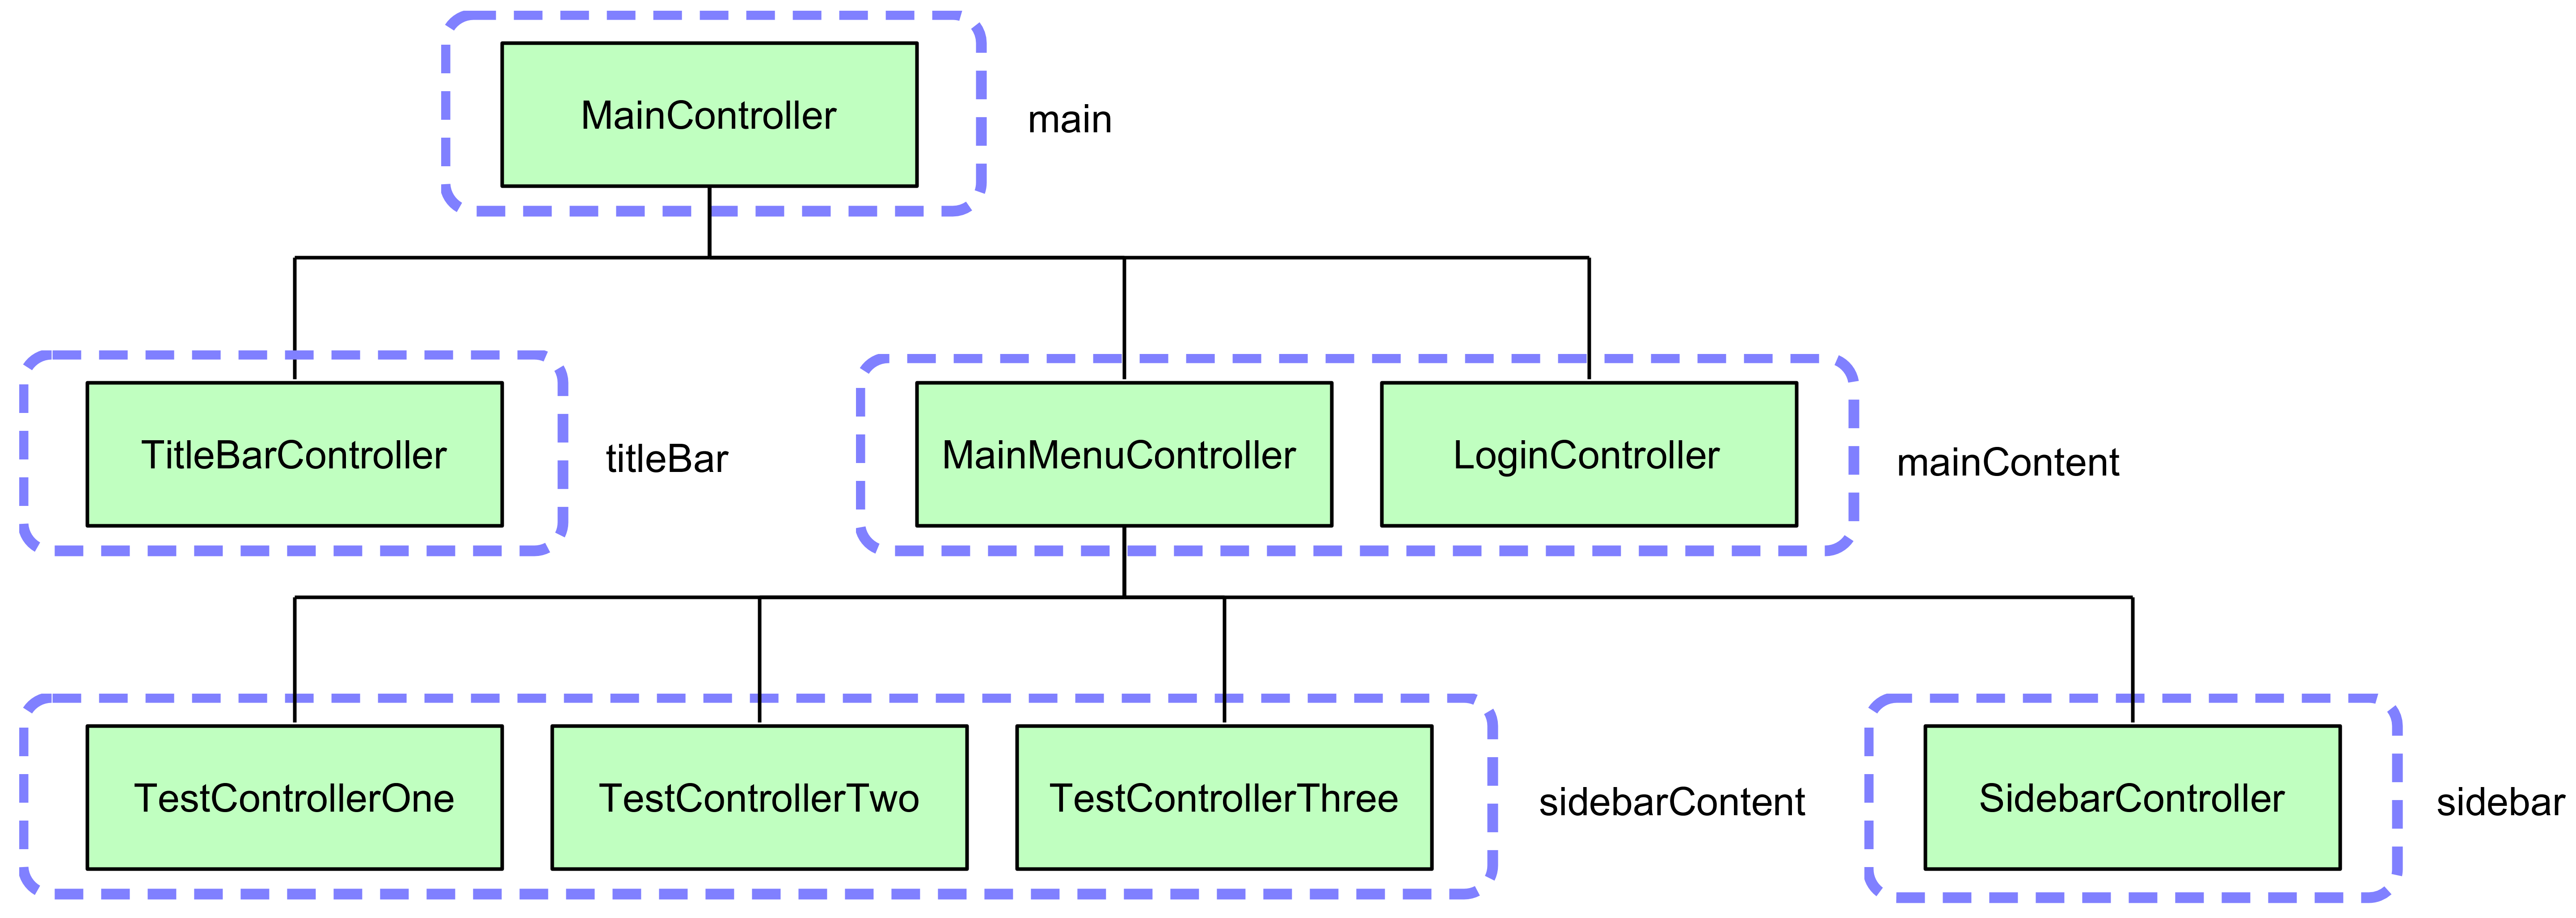
\includegraphics[width=\textwidth]{Abbildungen/Controller Relations.png}
	\caption{Diagramm -- Controller und Controllergruppen}
	\label{fig:controller_relations}
\end{figure}
\subsection{Implementierung der Beispielanwendung}
Damit eine \texttt{SimpliFX} Anwendung als solche erkannt wird, muss eine Klasse definiert werden, welche als Einstiegspunkt dienen soll. Diese muss die Annotation \texttt{@ApplicationEntryPoint} aufweisen und als Parameter den Startcontroller (\texttt{MainController}) übergeben. Für die Abhängigkeitsinjektion mit Guice muss der Einstiegspunkt auch mit \texttt{@GuiceInjection} annotiert werden und die Klasse eines Guice-Moduls übergeben. Wie in der Einleitung bereits beschrieben, wird das Modul nur die Implementierung des Login Services bereitstellen (siehe \autoref{fig:login_service}). 
\begin{figure}[H]
	\centering
	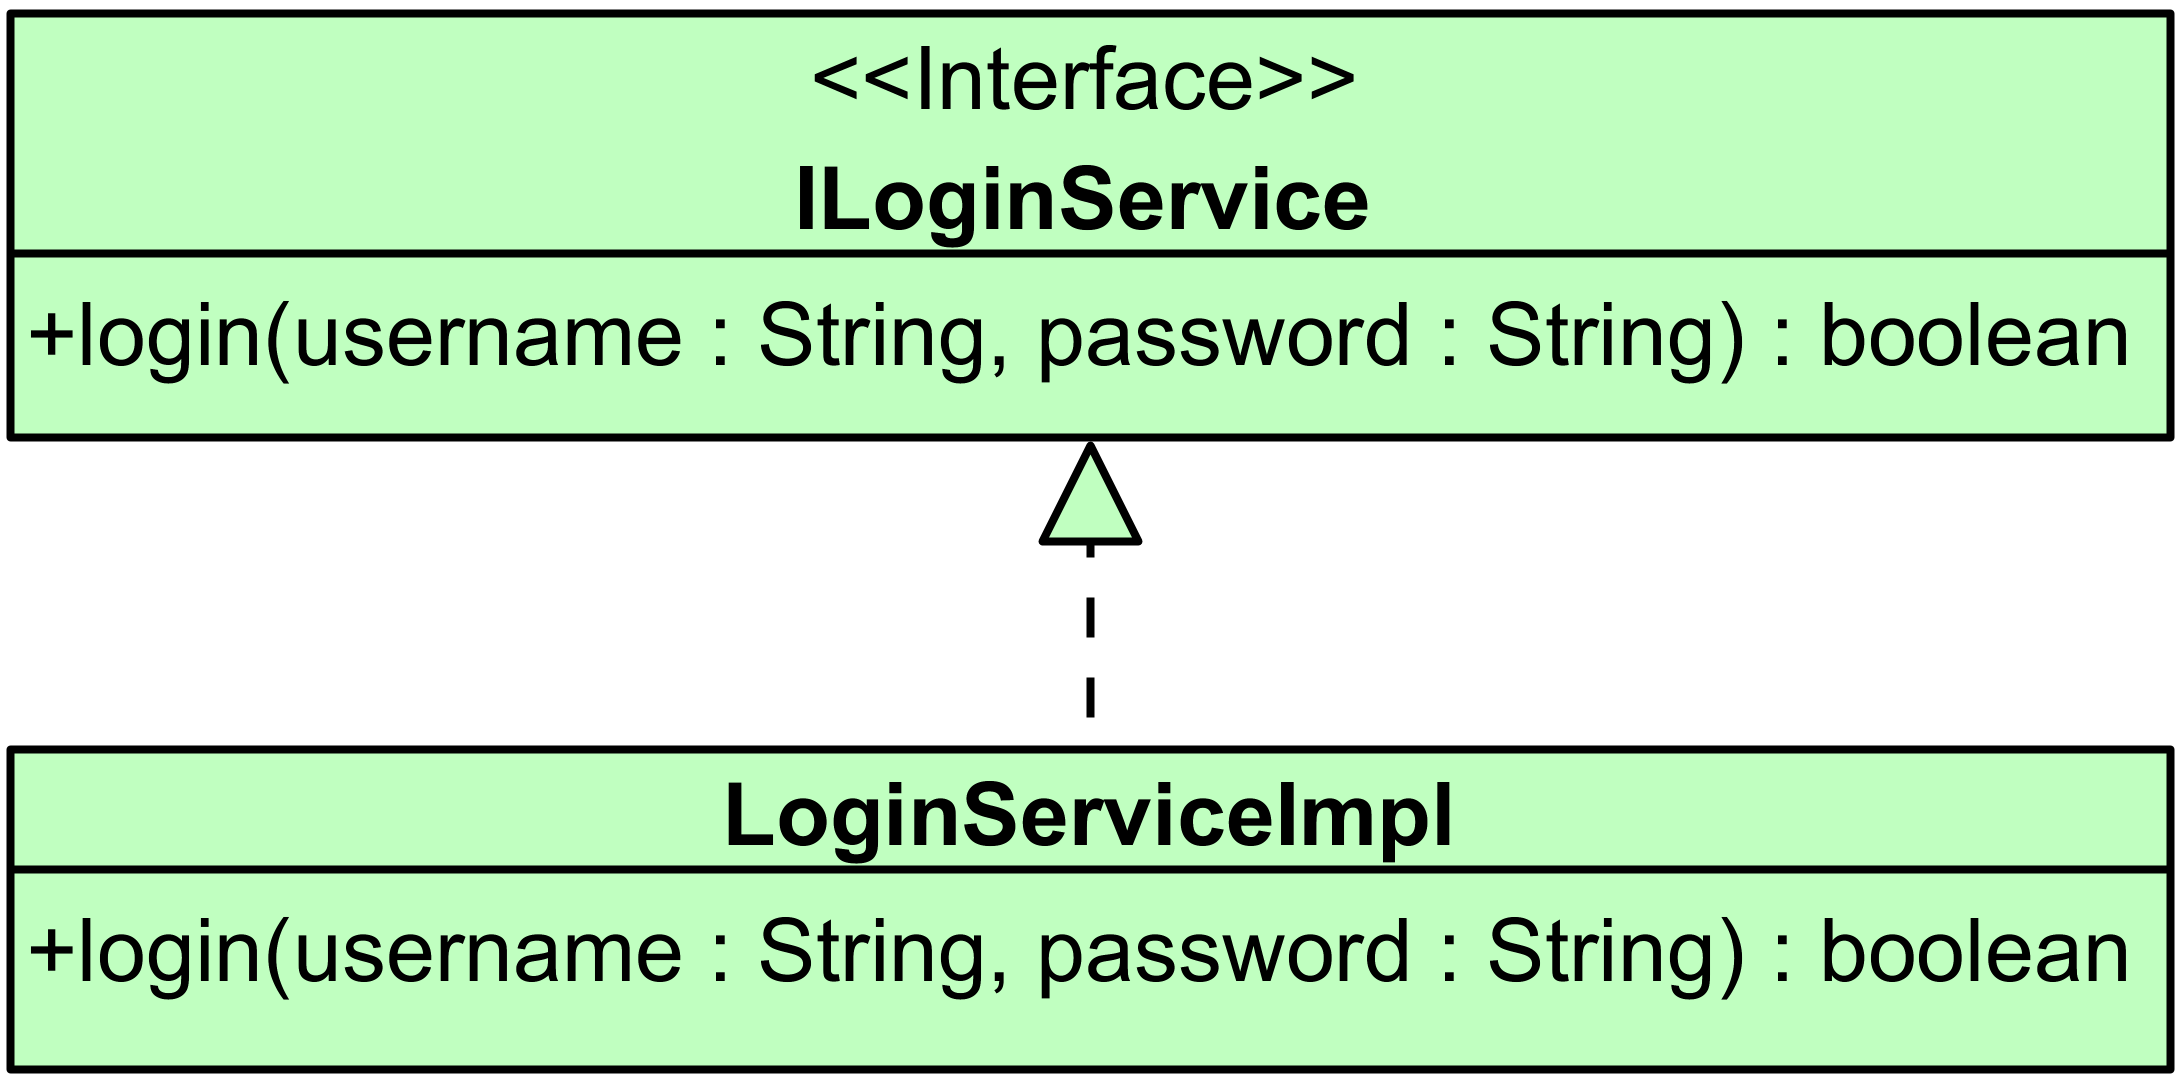
\includegraphics[width=\textwidth]{Abbildungen/Login Service.png}
	\caption{Diagramm -- Login Service}
	\label{fig:login_service}
\end{figure}
\noindent Dazu werden noch Konfigurationsänderungen der \texttt{Stage} in Form von Symbol- und Titeländerungen durchgeführt. Eine minimale Version des Einstiegspunktes ist in \autoref{lst:entry_point_demo} zu sehen. Dabei wird in der ersten Zeile der Titel der \texttt{Stage} auf \texttt{Login} gesetzt und ein Symbol für die Fensterleiste angegeben. Danach wird der Hauptcontroller in der zweiten Zeile definiert, indem die jeweilige Controllerklasse als Parameter übergeben wird. Abschließend wird die Guice Kompatibilität aktiviert und ein Modul festgelegt (Zeile drei).
\begin{figure}[H]
	\begin{lstlisting}[caption=Demo -- Minimaler Einstiegspunkt, captionpos=b, label=lst:entry_point_demo, numbers=left, xleftmargin=1.5em, framexleftmargin=1.5em]
#@StageConfig(title = "Login", icons = "icon.png")
#@ApplicationEntryPoint(MainController.class)
#@GuiceInjection(MainModule.class)
public final class DemoApplication {}
	\end{lstlisting}
\end{figure}
\noindent Für das Nutzen der dynamischen Übersetzung und der Konfigurationsschnittstelle müssen dem Einstiegspunkt zwei Felder hinzugefügt werden (\autoref{lst:fields_demo}). Außerdem sollen Subcontroller die Möglichkeit haben, den Titel der \texttt{Stage} abzuändern, weshalb die \texttt{titleProperty} als geteilte Ressource definiert wird und beim Start der Anwendung in einer \texttt{EventHandler} Methode gesetzt wird (\autoref{lst:event_method_demo}).
\begin{figure}[H]
	\begin{lstlisting}[caption=Demo -- Benötigte Felder, captionpos=b, label=lst:fields_demo]
#@ResourceBundle((@\tikzmark{resLeft}{}@)"lang.Messages"(@\tikzmark{resRight}{}@))
private II18N ii18N;

#@ConfigSource((@\tikzmark{conLeft}{}@)"config/connection"(@\tikzmark{conRight}{}@))
private Properties properties;

#@Shared
private SharedReference<StringProperty> (@\tikzmark{titleLeft}{}@)titleRef(@\tikzmark{titleRight}{}@);(@\begin{tikzpicture}[overlay,remember picture]
	\node[draw](resources) at (-0.5,3) {Pfad zum ResourceBundle};
	\node[draw](config) at (0.4,2) {Pfad zur Konfigurationsdatei};
	\node[draw](title) at (0.4,1) {Geteilte Ressource für Titel};
	\foreach \x/\y in {con/red,title/blue} {
		\DrawOverBar[-,\y,thick]{\x Left.north}{\x Right.north}
	}
	\DrawArrow[blue, in=280, out=-280]{title}{title}{0,-0.2}
	\DrawArrow[red, in=150, out=10]{con}{config}{-3.05,0.0}
	\renewcommand{\VerticalShiftForBar}{0em, -1.6ex}
	\renewcommand{\Stub}{0em, 0.3em}
	\DrawOverBar[-, green, thick]{resLeft.north}{resRight.north}
	\renewcommand{\VerticalShiftForArrows}{0, -1ex}
	\DrawArrow[green, in=215, out=-10]{res}{resources}{-2.3,-0.25}

\end{tikzpicture}@)
	\end{lstlisting}
\end{figure}
\begin{figure}[H]
	\begin{lstlisting}[caption=Demo -- Start EventHandler, captionpos=b, label=lst:event_method_demo]
#@EventHandler
private void onStart(StartEvent event) {
	// Titel Property setzen
    this.titleRef.set(event.getStage().titleProperty());
	// Stage zeigen
    event.getStage().show();
}
	\end{lstlisting}
\end{figure}
\noindent Zum Starten der Anwendung muss der Hauptcontroller korrekt deklariert werden und eine \texttt{main} Methode existieren, welche \texttt{SimpliFX\#launch} aufruft. Außerdem muss, aufgrund der Inkompatibilität zwischen JFoenix und Java 16, per Reflection-Schnittstelle eine \texttt{add-opens} Direktive vor der eigentlichen Initialisierung von \texttt{SimpliFX} und \texttt{JavaFX} hinzugefügt werden.\footnote{JFoenix Issue: \url{https://github.com/sshahine/JFoenix/issues/1052}} Der Einfachheit halber wird die \texttt{main} Methode in der \texttt{DemoApplication} Klasse definiert (\autoref{lst:main_method_demo}).
\begin{figure}[H]
\begin{lstlisting}[caption=Demo -- \texttt{main} Methode, captionpos=b, label=lst:main_method_demo]
public static void main(String[] args) throws Exception {
    Reflection.addOpens("java.lang.reflect", "java.base",
			JFXTextFieldSkin.class.getModule());
    SimpliFX.launch();
}
	\end{lstlisting}
\end{figure}
\noindent Der funktionsfähige Einstiegspunkt der Anwendung ist noch einmal vollständig in \autoref{lst:entry_point_demo_full} dargestellt.\\
Wird zu diesem Zeitpunkt versucht, die Applikation zu starten, wird diese mit einem Fehler terminieren, da der angegebene Hauptcontroller noch nicht erstellt und konfiguriert wurde.
Für eine valide Konfiguration muss die \texttt{MainController} Klasse die \texttt{@Controller} Annotation aufweisen, sowie mindestens den Pfad zu einer FXML Datei als Parameter enthalten. Außerdem wird für das Design des Layouts eine globale \ac{css} Datei angegeben. In \autoref{lst:main_controller_demo} ist der Klassenkopf des Hauptcontrollers mit allen nötigen Konfigurationen der Annotation abgebildet.\footnote{Für alle weiteren Controller wird der Klassenkopf, aufgrund der fast identischen Struktur, weggelassen.}
\begin{figure}[H]
	\begin{lstlisting}[caption=Demo -- \texttt{MainController} Klassenkopf, captionpos=b, label=lst:main_controller_demo]
#@Controller(fxml = "/fxml/MainController.fxml", 
#					 css = "css/main.css")
public final class MainController {}
	\end{lstlisting}
\end{figure}
\noindent Das Wurzelelement ist eine \texttt{BorderPane}, welche in der Setup-Phase des Controllers mit der \texttt{titleBar} und \texttt{mainContent} Untergruppe initialisiert wird. Erstere Gruppe findet ihren Ursprung im oberen Teil und letztere im mittleren Bereich der \texttt{BorderPane}. Das Setzen der Elemente zur Aufbauphase wird in \autoref{lst:main_controller_setup} gezeigt.
\begin{figure}[H]
	\begin{lstlisting}[caption=Demo -- \texttt{MainController} Setup-Phase, captionpos=b, label=lst:main_controller_setup]
#@FXML
private BorderPane root;

#@Setup
private void setup(ControllerSetupContext ctx) {
	// Erstelle Untergruppe "titleBar" mit TitleBarController 
	// als Startcontroller
    ctx.createSubGroup(TitleBarController.class, "titleBar", 
			this.root::setTop);
	// Erstelle Untergruppe "mainContent" mit LoginController
	// als Startcontroller
    ctx.createSubGroup(LoginController.class, "mainContent",
			this.root::setCenter);
}
	\end{lstlisting}
\end{figure}
\noindent Der vollständige Quelltext des Hauptcontrollers ist in \autoref{lst:main_controller} zu finden. Die Höhe und die Breite einer Controllergruppe richtet sich immer nach dem Startcontroller dieser. \texttt{SimpliFX} nutzt dazu das \texttt{prefHeight}- und \texttt{prefWidth}-Attribut des jeweiligen Wurzelelementes. Ist kein solches Attribut gesetzt worden, werden Standardwerte genutzt.\\
Der für das Ändern der Sprache verantwortliche \texttt{TitleBarController} benötigt ein JavaFX \texttt{Menu}, welches durch die FXML Datei zur Verfügung gestellt wird und eine PostConstruct Methode, welche dieses initialisiert (\autoref{lst:titlebar_controller_content}).
\begin{figure}[H]
	\begin{lstlisting}[caption=Demo -- Felder und Methoden im \texttt{TitleBarController}, captionpos=b, label=lst:titlebar_controller_content]
#@FXML
private Menu languageMenu;

#@ResourceBundle
private II18N ii18N;

#@PostConstruct
private void initMenu() {
    this.ii18N.setupMenu(this.languageMenu);
}
	\end{lstlisting}
\end{figure}
\noindent Der \texttt{LoginController} übernimmt die Aufgabe eines Loginvorgangs bei einem imaginären Server. Die Zugangsdaten zu ebendiesem sind in der Konfigurationsdatei enthalten, welche im Einstiegspunkt der Anwendung mit \texttt{SimpliFX} verbunden wurde. Die Eingabefelder für den Benutzernamen und das Passwort werden durch den \texttt{SimpliFXMLLoader}, der \texttt{ILoginService} durch Guice und verschiedene geteilte Ressourcen durch \texttt{SimpliFX} in den Controller injiziert (siehe \autoref{lst:login_controller_fields}). Das \texttt{titleRef} Feld wird aufgrund des Feldnamens die gleiche geteilte Ressource erhalten, welche in \autoref{lst:fields_demo} deklariert wurde.
\begin{figure}[H]
	\begin{lstlisting}[caption=Demo -- Injizierte Felder des \texttt{LoginController}s, captionpos=b, label=lst:login_controller_fields]
#@FXML
private JFXTextField usernameField;

#@FXML
private JFXPasswordField passwordField;

#@Shared
private SharedReference<String> usernameRef;

#@Shared
private SharedReference<StringProperty> titleRef;

#@Inject
private ILoginService loginService;
	\end{lstlisting}
\end{figure}
\noindent Damit der Titel der \texttt{Stage} geändert wird sobald der \texttt{LoginController} angezeigt wird, muss eine Methode erstellt werden, welche bei der OnShow-Phase aufgerufen wird und dabei den eigentlichen Titel abändert. Des Weiteren müssen die Textfelder für das Eingeben des Benutzernamens und des Passwortes bei einem Verstecken des Controllers aus Sicherheitsgründen gelöscht werden. Analog zur ersteren Methode kann dies in der \texttt{OnHide} Phase erfolgen (siehe \autoref{lst:login_controller_visibility_methods}).
\begin{figure}[H]
	\begin{lstlisting}[caption=Demo -- OnShow und OnHide Methoden, captionpos=b, label=lst:login_controller_visibility_methods]
#@OnShow
private void onShow() {
    this.titleRef.get().set("Login");
}

#@OnHide
private void onHide() {
    this.usernameField.clear();
    this.passwordField.clear();
}
	\end{lstlisting}
\end{figure}
\noindent Zu diesem Zeitpunkt kann die Anwendung das erste Mal ohne einen Konfigurationsfehler gestartet werden. Der aktuelle Stand der Applikation ist in \autoref{fig:login_controller_demo} dargestellt. Alle bis hierhin verwendeten Controller wurden hervorgehoben.
\begin{figure}[H]
	\centering
	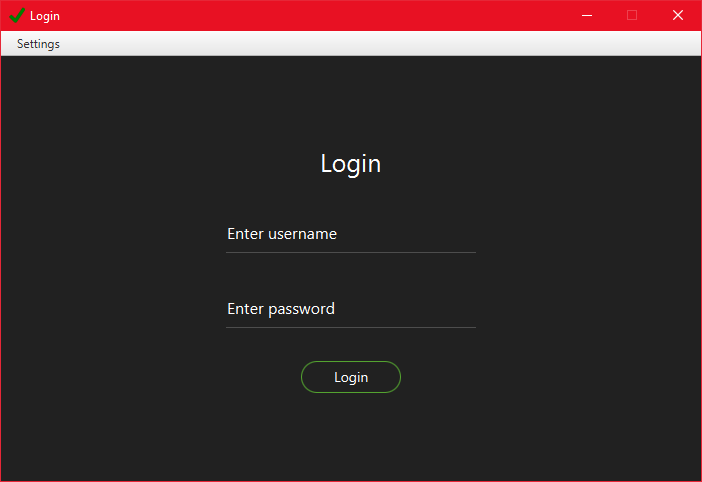
\includegraphics[width=\textwidth]{Abbildungen/Login Screen.png}
	\caption{Diagramm -- Erster Start der Anwendung.}
	\label{fig:login_controller_demo}
\end{figure}
\noindent Nach einem Login muss der aktive Controller der \texttt{mainContent} Gruppe zum \texttt{MainMenuController} gewechselt werden. Dazu muss der \texttt{LoginController} zur Setup-Phase den \texttt{ControllerSetupContext} speichern und bei einem Klick auf die Login-Schaltfläche einen Wechsel initiieren. Die dafür nötigen Erweiterungen der Klasse sind in \autoref{lst:login_controller} abgebildet. Der \texttt{MainMenuController} kapselt eine \texttt{BorderPane}, welche im linken Bereich die \texttt{sidebar} und im Mittelbereich die \texttt{sidebarContent} Gruppe darstellt (\autoref{lst:mainmenu_controller_setup}). Bei einem Wechsel soll der Stagetitel den aktuell eingeloggten Nutzer begrüßen. Die dafür benötigten Felder und Methoden sind in der vollständigen Implementierung der Klasse zu finden (\autoref{lst:mainmenu_controller}).
\begin{figure}[H]
	\begin{lstlisting}[caption=Demo -- Subgruppen Einrichtung, captionpos=b, label=lst:mainmenu_controller_setup]
#@FXML
private BorderPane root;

#@FXML
private StackPane contentCenter;

#@Setup
private void setup(ControllerSetupContext ctx) {
    ctx.createSubGroup(SidebarController.class, "sidebar",
			this.root::setLeft);
    ctx.createSubGroup(TestControllerOne.class, "sidebarContent",
			this.contentCenter.getChildren()::setAll);
}
	\end{lstlisting}
\end{figure}
\noindent Die \texttt{sidebarContent} Gruppe beinhaltet drei mögliche Controller, von welchen keiner besondere Methoden oder Felder benötigt und ein leerer Klassenrumpf teilweise für Testzwecke genügt. Aus Vollständigkeitsgründen sind diese dennoch in \autoref{lst:test_controllers} dargestellt.\\
Der \texttt{SidebarController} setzt sich aus zwei Komponenten zusammen:
\begin{itemize}
	\item Die Serveranzeige, welche den aktuellen Server aus der Konfigurationsdatei anzeigt und per \texttt{@LocalizeValue} aktualisiert werden kann.
	\item Die Schaltflächengruppe, welche für das Wechseln des aktuellen Controllers der \texttt{sidebarContent} Gruppe zuständig ist und ein Ausloggen ermöglicht. Beim Ausloggen wird dabei zum \texttt{LoginController} gewechselt.
\end{itemize}
Das Verwenden der \texttt{@LocalizeValue} und der \texttt{@ConfigValue} Annotation wird im Folgenden beispielhaft anhand des Hostnamens demonstriert (\autoref{lst:sidebar_controller_localize}).
\begin{figure}[H]
	\begin{lstlisting}[caption=Demo -- \texttt{@LocalizeValue} und \texttt{@ConfigValue}, captionpos=b, label=lst:sidebar_controller_localize]
#@FXML
private Label connectionLbl;

#@ConfigValue("host")
private String hostname;

#@LocalizeValue(id = "connectionLbl", property = "text")
private StringProperty hostProperty = new SimpleStringProperty();
	\end{lstlisting}
\end{figure}
\noindent Nach der Konstruktion des Controllers muss der Stringwert der \texttt{hostProperty} geändert werden, um die \texttt{textProperty} des \texttt{connectionLbl} Labels mit dem aktuellen Hostnamen zu aktualisieren. Die Implementierung der Seitenleiste ist in \autoref{lst:sidebar_controller} und der aktuelle Zustand der Anwendung nach dem Loginvorgang in \autoref{fig:mainmenu_controller_demo} dargestellt.
\begin{figure}[H]
	\centering
	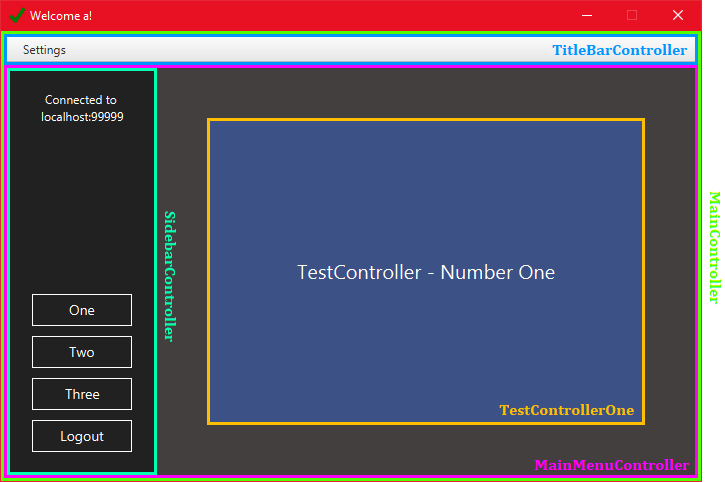
\includegraphics[width=\textwidth]{Abbildungen/MainMenu Screen.png}
	\caption{Diagramm -- Anwendung nach Login}
	\label{fig:mainmenu_controller_demo}
\end{figure}
\section{Evaluation der Bibliothek}
Viele der implementierten Funktionen erweitern den Funktionsumfang von JavaFX und lassen sich somit nicht direkt vergleichen. Im Folgenden werden einzelne Aspekte von \texttt{SimpliFX} denen von JavaFX gegenübergestellt und mögliche Vereinfachungen oder Restriktionen aufgezeigt.
\subsection{Start der Anwendung}
Der Start der Anwendung erfolgt ähnlich wie in JavaFX. Dabei wurde die interne JavaFX Launcher Implementierung vollständig durch eine eigene ersetzt, was in mehr Freiheiten bei der Applikationsinitialisierung resultiert. So ist es nun möglich, bereits initialisierte Applikationsklassen als Einstiegspunkt zuzulassen, da eine manuelle Instanziierung nicht mehr durch den Launcher vorausgesetzt ist. Dazu kann der Entwickler die Preloaderfunktion verwenden, ohne interne JavaFX Methoden aufrufen zu müssen. Des Weiteren wird der Einstiegspunkt sowohl für die Applikation als auch für den Preloader automatisch durch das Durchsuchen des Klassenpfades gefunden. Ein manuelles Angeben der Klassen ist dabei nicht mehr notwendig, sondern optional. Problematiken bei der Nutzung von JavaFX mit Apache Maven, welche auf die Jigsaw API zurückzuführen sind, werden durch \texttt{SimpliFX} verhindert. Die eigene Implementierung der Launcherklasse für den Anwendungsstart und das Initialisieren der JavaFX Plattform weist jedoch auch Nachteile auf. Beispielsweise wird bei in der \texttt{Application\#notifyPreloader} Methode weiterhin die interne Launcher Implementierung verwendet, weshalb ein Aufruf dieser keinen Einfluss auf den von \texttt{SimpliFX} genutzten Preloader hat.
\subsection{Einstiegspunkte}
Die Einstiegspunkte ermöglichen eine einfache, automatische Konfiguration der \texttt{Stage} durch das Verwenden von Annotationen. Dazu sind die eventbasierten Methoden für das Behandeln des Applikations- bzw. Preloader-Lebenszyklus vollständig optional und können im Gegensatz zu JavaFX weggelassen werden. Eine vollständig funktionsfähige Anwendung kann mit nur zwei Klassen (Einstiegspunkt, Hauptcontroller) und drei Annotationen (ApplicationEntryPoint, StageConfig, Controller) realisiert werden. Ausnahmen, welche auf dem JavaFX-Thread, in Lebenszyklusmethoden oder dem Einrichten von Subsystemen auftreten, können an den Preloader weitergeleitet und durch ebendiesen behandelt werden. 
\subsection{Lokalisierung}
Die Lokalisierungsmöglichkeiten in JavaFX sind strukturell durch die Implementierung des \texttt{FXMLLoader}s limitiert. Der herkömmliche \texttt{FXMLLoader} erlaubt das einmalige Übersetzen in Form von Stringwerten beim Laden einer FXML Datei und verhindert somit die dynamische Änderung der Sprache ohne ein vollständiges Neuladen der jeweiligen betroffenen Dateien. Diese Limitation wurde durch den \texttt{SimpliFXMLLoader} entfernt, indem die Übersetzung nun in Form von aktualisierbaren \texttt{StringBinding} Instanzen durchgeführt wird. Auch ist die Unterstützung von parametrisierten Übersetzungsschlüsseln bei der Verwendung von JavaFX oder \texttt{SimpliFX} Controllern ermöglicht worden. Weiterhin können die Lokalisierungsschnittstelle und der \texttt{SimpliFXMLLoader} auch außerhalb vom Controller-System eigenständig genutzt werden.
\subsection{Controller}
Controller von \texttt{SimpliFX} erlauben eine Verschachtelung sowie eine Gruppierung und wurden um einen Lebenszyklus erweitert. Sie können beliebig oft mit oder ohne Verwendung von Animationen gewechselt werden und sind in der Lage, Lebenszyklusänderungen an eventuelle Untercontroller zu delegieren. Außerdem ist es möglich verschiedene Objekte als geteilte Ressourcen zu definieren, welche von allen aktiven Controllern genutzt werden können. Eine Änderung dieser wird auf alle anderen Controller reflektiert. Jede Controllergruppe ist dabei im Stande Benachrichtigungen anzuzeigen. Der Entwickler kann das Layout dieser vollständig kontrollieren oder das Standardlayout verwenden.
\subsection{Abhängigkeitsinjektion}
JavaFX besitzt keine direkte Möglichkeit für eine Abhängigkeitsinjektion durch etablierte, externe Bibliotheken. \texttt{SimpliFX} bringt dieses Konzept in die JavaFX Umgebung und ermöglicht somit das Verwenden solcher Bibliotheken in allen Controllern und Einstiegspunkten. Soll eine Bibliothek verwendet werden, welche nicht direkt durch \texttt{SimpliFX} bereitgestellt wird, kann diese mit wenig Zeitaufwand hinzugefügt werden.
\subsection{Konfigurationsdateien}
Alle Konfigurationsdateien, welche eine Kompatibilität mit der Java Properties API aufweisen, können durch \texttt{SimpliFX} aus dem Klassenpfad sowie aus externen Quellen geladen und den Einstiegspunkten und Controllern zur Verfügung gestellt werden. Dabei ist die Verwendung von Standardwerten möglich, wenn Konfigurationsschlüssel nicht in den angegebenen Konfigurationsdateien gefunden werden können.